% =============================================================================
% Оформление пособия — «лётный журнал инструктора».
% Палитра и гарнитуры совпадают с веб-симулятором (simulator/DESIGN.md):
% графит #162235, оранжевый #ff6b00, светлые нейтральные поверхности, Inter.
% Классы документа и опции — в main.tex; здесь шрифты, цвета, рамки, титул.
% =============================================================================

% --- Язык и шрифты (XeLaTeX) --------------------------------------------------
\usepackage{fontspec}
\usepackage{polyglossia}
\setdefaultlanguage{russian}
\setotherlanguage{english}

% Всё из TeX Live: книга собирается одинаково на любой машине.
\setmainfont{XCharter}[Ligatures=TeX]
\setsansfont{Inter}[Ligatures=TeX, Scale=0.97]
\newfontfamily\cyrillicfontsf{Inter}[Ligatures=TeX, Scale=0.97] % у Inter нет тега скрипта cyrl
\setmonofont{CascadiaCode-Regular.otf}[BoldFont=CascadiaCode-Bold.otf, ItalicFont=CascadiaCode-Italic.otf, BoldItalicFont=CascadiaCode-BoldItalic.otf, Scale=MatchLowercase, RawFeature={-calt}]
\newfontfamily\codefont{CascadiaCode-Regular.otf}[BoldFont=CascadiaCode-Bold.otf, ItalicFont=CascadiaCode-Italic.otf, BoldItalicFont=CascadiaCode-BoldItalic.otf, Scale=MatchLowercase, RawFeature={-calt}]

\usepackage{microtype}
\emergencystretch=3em
\sloppy

% Абзацы: без красной строки, воздух между абзацами (parskip=half задан в main.tex).
\usepackage{setspace}
\setstretch{1.1}

% --- Математика ---------------------------------------------------------------
\usepackage{amsmath}
\usepackage{amssymb}

% --- Цвета ---------------------------------------------------------------------
\usepackage[table]{xcolor}
\definecolor{Ink}{HTML}{162235}        % основной текст и заголовки
\definecolor{Muted}{HTML}{647286}      % подписи, второстепенное
\definecolor{Rule}{HTML}{DDE3EA}       % линии и тонкие рамки
\definecolor{Paper}{HTML}{F7F7F5}      % поверхности под кодом и таблицами
\definecolor{Orange}{HTML}{FF6B00}     % действие, акцент (заливки)
\definecolor{Accent}{HTML}{C95E09}     % акцент в тексте (контраст на белом)
\definecolor{Success}{HTML}{17794D}    % «получилось», миссии
\definecolor{Danger}{HTML}{C23428}     % ошибки и опасность
\definecolor{InfoBlue}{HTML}{2D5A8A}   % справка и ссылки
% прежние имена — чтобы не переписывать главы и рисунки
\colorlet{GeoskanDarkBlue}{Ink}
\colorlet{GeoskanBlue}{InfoBlue}
\colorlet{GeoskanOrange}{Orange}
\colorlet{GeoskanMuted}{Muted}
\colorlet{GeoskanLightGray}{Paper}
\colorlet{CodeBack}{Paper}
\colorlet{TaskTeal}{Success}
\definecolor{CodeGreen}{RGB}{0, 150, 0}
\definecolor{CodePurple}{RGB}{128, 0, 128}
% цвета рисунков дрона (tikz_drone)
\definecolor{GeoskanBlack}{RGB}{30, 30, 35}
\definecolor{GeoskanDarkGrey}{RGB}{45, 45, 50}
\definecolor{GeoskanGrey}{RGB}{100, 100, 105}
\definecolor{GeoskanLightGrey}{RGB}{180, 180, 185}
\definecolor{SkyTop}{RGB}{100, 180, 255}
\definecolor{SkyBottom}{RGB}{200, 230, 255}
\definecolor{GroundGreen}{RGB}{34, 139, 34}
\color{Ink}

\usepackage{graphicx}
\graphicspath{{images/}{chapters/python/images/}}
\usepackage{float}
\usepackage{adjustbox}
\usepackage{tikz}
\usepackage{tikz-3dplot}
\usetikzlibrary{arrows.meta, quotes, 3d, calc, shapes.geometric, shadows, positioning, decorations.markings, fadings, patterns, shadings, shapes, babel}
\tikzfading[name=fade out, inner color=transparent!0, outer color=transparent!100]

% --- Библиография ------------------------------------------------------------
\usepackage[
    backend=biber,
    style=gost-numeric,
    language=auto,
    autolang=other,
    sorting=none
]{biblatex}
\addbibresource{styles/references.bib}

% --- Страница -----------------------------------------------------------------
\usepackage{geometry}
\geometry{
    a4paper,
    top=27mm,
    bottom=24mm,
    left=27mm,
    right=27mm,
    headheight=14pt,
    headsep=9mm,
    footskip=12mm
}

% --- Колонтитулы: название главы слева, номер страницы справа -----------------
\usepackage[automark, headsepline=0.4pt]{scrlayer-scrpage}
\clearpairofpagestyles
\ihead{\headmark}
\ohead{\pagemark}
\setkomafont{pageheadfoot}{\sffamily\footnotesize\color{Muted}}
\setkomafont{pagenumber}{\sffamily\bfseries\color{Accent}}
\addtokomafont{headsepline}{\color{Rule}}
\makeatletter
\renewcommand*{\sectionmarkformat}{\thesection\enskip}
\makeatother

% --- Заголовки -------------------------------------------------------------------
% Глава: метка «ГЛАВА N» оранжевым, название крупно, короткая оранжевая черта.
\setkomafont{section}{\sffamily\bfseries\fontsize{25}{29}\selectfont\color{Ink}}
\renewcommand*{\sectionformat}{\thesection}
\makeatletter
\renewcommand*{\sectionlinesformat}[4]{%
    \ifstrequal{#1}{section}{%
        \parbox[t]{\linewidth}{\raggedright\setlength{\parskip}{0pt}%
            \ifstrempty{#3}{}{{\sffamily\footnotesize\bfseries\color{Accent}\addfontfeature{LetterSpace=14}ГЛАВА\enspace#3}\par\vspace{6pt}}%
            #4\par\vspace{7pt}%
            {\color{Orange}\rule{3.4cm}{2.4pt}}}%
    }{\@hangfrom{\hskip #2#3}#4}%
}
\makeatother
\RedeclareSectionCommand[beforeskip=0pt,afterskip=1.4em]{section}
\AddToHook{cmd/section/before}{\clearpage}

\setkomafont{subsection}{\sffamily\bfseries\fontsize{15}{19}\selectfont\color{Ink}}
\renewcommand*{\subsectionformat}{{\color{Accent}\thesubsection}\enskip}
\setkomafont{subsubsection}{\sffamily\bfseries\fontsize{12}{15}\selectfont\color{Ink}}
\renewcommand*{\subsubsectionformat}{{\color{Muted}\thesubsubsection}\enskip}
\setkomafont{paragraph}{\sffamily\bfseries\color{Ink}}
\RedeclareSectionCommand[beforeskip=1.9em plus .3em minus .2em,afterskip=.7em]{subsection}
\RedeclareSectionCommand[beforeskip=1.4em plus .2em minus .1em,afterskip=.45em]{subsubsection}

% Часть: тёмная страница, крупное название.
\setkomafont{part}{\sffamily\bfseries\fontsize{36}{42}\selectfont\color{white}}
\setkomafont{partnumber}{\sffamily\bfseries\fontsize{13}{17}\selectfont\color{Orange}}
\renewcommand*{\partformat}{%
    \begin{tikzpicture}[remember picture,overlay]
        \fill[Ink] (current page.south west) rectangle (current page.north east);
    \end{tikzpicture}%
    \addfontfeature{LetterSpace=16}ЧАСТЬ\enspace\thepart}
\renewcommand*{\raggedpart}{\raggedright}
\renewcommand*{\partheadstartvskip}{\vspace*{0.24\textheight}}
\renewcommand*{\partheadmidvskip}{\par\vspace{14pt}}
\renewcommand*{\partheadendvskip}{\par\vspace{14pt}{\color{Orange}\rule{3.4cm}{2.4pt}}\par}
\setcounter{tocdepth}{2}

% --- Списки и таблицы ---------------------------------------------------------
\usepackage{enumitem}
\setlist{nosep, topsep=0.35em, itemsep=2pt plus 1pt}
\setlist[itemize]{label=\textcolor{Orange}{\textbullet}, leftmargin=1.3em}
\setlist[enumerate]{label=\textcolor{Accent}{\sffamily\bfseries\small\arabic*.}, leftmargin=1.7em}
\setlist[description]{font=\sffamily\bfseries\color{Ink}}

\usepackage{booktabs}
\setlength{\heavyrulewidth}{0.8pt}
\setlength{\lightrulewidth}{0.4pt}
\arrayrulecolor{Ink!60}
\renewcommand{\arraystretch}{1.3}
\usepackage{tabularx}
\usepackage{multirow}
\usepackage{longtable}
\usepackage{caption}
\captionsetup{font={small,color=Muted}, labelfont={bf,sf,color=Accent}, labelsep=period, singlelinecheck=false, skip=6pt}

% --- Листинги (minted2: подсветка через pygmentize по \write18) --------------------
\usepackage[outputdir=../build]{minted2}
\usemintedstyle{friendly}
\setminted{fontsize=\footnotesize, breaklines=true, breakafter={,(}, frame=none, baselinestretch=1.0, linenos=false}

% --- Рамки -------------------------------------------------------------------------
\usepackage{tcolorbox}
\usepackage{etoolbox}
\tcbuselibrary{skins, breakable}
\usepackage{fontawesome5}
\usepackage{textcomp}
\usepackage{accsupp}
\usepackage{attachfile2}
\providecommand{\faPencilAlt}{\faPen}

% Копируемый код: точная копия исходника через /ActualText (см. codeacc.tex).
% --- Copy-paste friendly code listings -------------------------------------
%
% Problem: the PDF text layer produced by minted/fancyvrb does not reproduce
% the original source file when the reader copies a listing out of the PDF:
%   * leading indentation is lost (spaces are TeX glue, not glyphs),
%   * the hyphen glyph is mapped to U+2010 instead of ASCII U+002D,
%   * a long line that visually wraps is copied as two lines and the
%     fvextra continuation symbol ",->" leaks into the copied text.
% All of that breaks the code as soon as it is pasted into the project's
% Monaco based web editor (and into any Lua/Python tool chain).
%
% Fix: read the real source file, and attach its exact text, line by line,
% to the typeset lines as a PDF /Span with /ActualText (accsupp).  Text
% extractors must honour /ActualText, so the copied text becomes the literal
% file content.  Nothing about the visual output changes.
%
% The ActualText deliberately carries NO line terminator: PDF viewers and
% extractors insert their own newline between two typeset lines, so adding
% U+000A here would produce doubled blank lines on paste.  Source lines that
% contain no visible glyph (empty or whitespace-only) get no span at all,
% because a marked-content span without glyphs confuses extractors.
%
% The previous \FV@Space patch (a single space wrapped in ActualText) was a
% no-op: with breaklines=true fvextra redefines \FV@Space when the listing
% environment starts, so the patch never reached the output.  It is replaced
% by the per-line mechanism below, which covers spaces as part of the line.

% accsupp's dvipdfm driver (the one XeTeX selects) emits BDC/EMC through the
% "pdf:content" special, which dvipdfmx wraps in "q <translate to the current
% point> cm ... Q".  Text extractors that compute the span's position at EMC
% time therefore see the span shifted to the right by the width of the line,
% which makes poppler place the whole listing in a bogus column and silently
% drop every listing after the first one on a page.  "pdf:code" injects the
% same operators with no transformation, which is what BDC/EMC need.
\makeatletter
\def\ACCSUPP@bdc{\special{pdf:code \ACCSUPP@span BDC}}
\def\ACCSUPP@emc{\special{pdf:code EMC}}
\makeatother

\ExplSyntaxOn
\seq_new:N  \g__codeacc_hex_seq
\int_new:N  \l__codeacc_index_int
\int_new:N  \l__codeacc_pending_int
\ior_new:N  \g__codeacc_ior
\bool_new:N \g__codeacc_active_bool
\tl_new:N   \l__codeacc_line_tl
\str_new:N  \l__codeacc_hex_str

% Store one raw source line as UTF-16BE hex (or an empty entry for a line
% that will not produce any glyph on the page).
\cs_new_protected:Npn \__codeacc_store_line:n #1
  {
    \tl_set:Nx \l__codeacc_line_tl { \tl_trim_spaces:n {#1} }
    \tl_if_empty:NTF \l__codeacc_line_tl
      {
        \int_incr:N \l__codeacc_pending_int
        \seq_gput_right:Nn \g__codeacc_hex_seq { }
      }
      {
        \str_set_convert:Nnnn \l__codeacc_hex_str {#1} { } { utf16be/hex }
        \seq_gput_right:Nx \g__codeacc_hex_seq { \str_use:N \l__codeacc_hex_str }
        \int_zero:N \l__codeacc_pending_int
      }
  }

% Read the whole source file once, before \inputminted typesets it.
\cs_new_protected:Npn \__codeacc_load:n #1
  {
    \seq_gclear:N \g__codeacc_hex_seq
    \bool_gset_false:N \g__codeacc_active_bool
    \file_if_exist:nT {#1}
      {
        \int_zero:N \l__codeacc_pending_int
        \ior_open:Nn \g__codeacc_ior {#1}
        \ior_str_map_inline:Nn \g__codeacc_ior { \__codeacc_store_line:n {##1} }
        \ior_close:N \g__codeacc_ior
        \bool_gset_true:N \g__codeacc_active_bool
      }
  }

% fvextra calls \FancyVerbFormatLine more than once per line (once inside a
% measuring \sbox), so the source line is looked up through fancyvrb's own
% FancyVerbLine counter instead of a counter of our own.
\cs_new_protected:Npn \__codeacc_wrap_line:n #1
  {
    \bool_if:NTF \g__codeacc_active_bool
      {
        \int_set:Nn \l__codeacc_index_int { \value{FancyVerbLine} }
        \str_set:Nx \l__codeacc_hex_str
          { \seq_item:Nn \g__codeacc_hex_seq { \l__codeacc_index_int } }
        \str_if_empty:NTF \l__codeacc_hex_str
          { #1 }
          {
            \exp_args:Nx \BeginAccSupp
              { method=hex,unicode,ActualText= \str_use:N \l__codeacc_hex_str }
            #1
            \EndAccSupp { }
          }
      }
      { #1 }
  }

% \CodeAccInputMinted{<language>}{<path relative to tex/>}
\NewDocumentCommand \CodeAccInputMinted { m m }
  {
    \__codeacc_load:n {#2}
    \group_begin:
      \cs_set_eq:NN \FancyVerbFormatLine \__codeacc_wrap_line:n
      \inputminted [ fontsize = \small ] {#1} {#2}
    \group_end:
  }
\ExplSyntaxOff


% Общий вид плашек: цветная полоса слева, лёгкая заливка, заголовок первой строкой.
% callout={цвет}{значок}{цвет заголовка}  — заголовок задаётся при вызове.
\tcbset{
    callout/.style n args={3}{
        enhanced, breakable, frame hidden, boxrule=0pt, arc=2pt, outer arc=2pt,
        colback=#1!7!white, colbacktitle=#1!7!white, coltitle=#3,
        borderline west={3pt}{0pt}{#1},
        fonttitle=\sffamily\bfseries\small, titlerule=0pt,
        left=9pt, right=9pt, top=6pt, bottom=6pt, toptitle=5pt, bottomtitle=0pt,
        before skip=0.9em plus 2pt, after skip=0.9em plus 2pt,
        title={\textcolor{#1}{#2}\enspace\ignorespaces},
    }
}

\newtcolorbox{infobox}[1][Информация]{callout={InfoBlue}{\faInfoCircle}{InfoBlue}, title={\textcolor{InfoBlue}{\faInfoCircle}\enspace #1}}
\newtcolorbox{warnbox}[1][Внимание]{callout={Danger}{\faExclamationTriangle}{Danger}, title={\textcolor{Danger}{\faExclamationTriangle}\enspace #1}}
\newtcolorbox{alertbox}[1][Важно]{callout={Danger}{\faExclamationCircle}{Danger}, title={\textcolor{Danger}{\faExclamationCircle}\enspace #1}}
\newtcolorbox{hintbox}[1][Подсказка]{callout={Orange}{\faLightbulb}{Accent}, title={\textcolor{Orange}{\faLightbulb}\enspace #1}}
\newtcolorbox{rulebox}[1][Правило]{callout={Ink}{\faGavel}{Ink}, title={\textcolor{Ink}{\faGavel}\enspace #1}}
\newtcolorbox{questionbox}[1][Вопрос]{callout={Success}{\faQuestionCircle}{Success}, title={\textcolor{Success}{\faQuestionCircle}\enspace #1}}
\newtcolorbox{missionbox}[1][Миссии симулятора]{callout={Success}{\faGamepad}{Success}, title={\textcolor{Success}{\faGamepad}\enspace #1}}

% Файл с кодом: полоса с путём сверху, под ней листинг.
\NewDocumentEnvironment{codefile}{O{python}m}{%
    \begin{tcolorbox}[
        enhanced, breakable, colback=Paper, colframe=Rule, boxrule=0.5pt, arc=2pt, outer arc=2pt,
        colbacktitle=Rule!60!white, coltitle=Ink, fonttitle=\ttfamily\scriptsize, toptitle=2pt, bottomtitle=2pt,
        left=3mm, right=3mm, top=2.5mm, bottom=2.5mm,
        before skip=0.9em plus 2pt, after skip=0.9em plus 2pt,
        title={\textcolor{Accent}{\faFileCode}\enspace\detokenize{#2}}
    ]
    \CodeAccInputMinted{#1}{../../examples/#2}
    \end{tcolorbox}
}{}
\NewDocumentEnvironment{codefiletitle}{O{python}mm}{%
    \begin{tcolorbox}[
        enhanced, breakable, colback=Paper, colframe=Rule, boxrule=0.5pt, arc=2pt, outer arc=2pt,
        colbacktitle=Rule!60!white, coltitle=Ink, fonttitle=\ttfamily\scriptsize, toptitle=2pt, bottomtitle=2pt,
        left=3mm, right=3mm, top=2.5mm, bottom=2.5mm,
        before skip=0.9em plus 2pt, after skip=0.9em plus 2pt,
        title={\textcolor{Accent}{\faFileCode}\enspace\detokenize{#2}}
    ]
    \CodeAccInputMinted{#1}{../../examples/#3}
    \end{tcolorbox}
}{}

% Короткий фрагмент кода прямо в тексте.
\newtcolorbox{codebox}[1][]{
    enhanced, breakable, colback=Paper, colframe=Rule, boxrule=0.5pt, arc=2pt,
    colbacktitle=Rule!60!white, coltitle=Ink, fonttitle=\sffamily\bfseries\scriptsize,
    left=3mm, right=3mm, top=2.5mm, bottom=2.5mm, title={#1}
}

% Задание после урока: заметный оранжевый заголовок «ЗАДАНИЕ 3.2 · Название».
% Внутри: \expected{что должно получиться} и \mission{Lua}{10--12}.
\newcounter{taskcounter}[section]
\renewcommand{\thetaskcounter}{\thesection.\arabic{taskcounter}}
\NewDocumentEnvironment{taskbox}{O{}}{%
    \refstepcounter{taskcounter}%
    \begin{tcolorbox}[
        enhanced, breakable, frame hidden, boxrule=0pt, arc=2pt, outer arc=2pt,
        colback=Orange!6!white, colbacktitle=Orange, coltitle=white,
        fonttitle=\sffamily\bfseries\small, titlerule=0pt, toptitle=3pt, bottomtitle=3pt,
        left=9pt, right=9pt, top=7pt, bottom=6pt,
        before skip=1.1em plus 3pt, after skip=1.1em plus 3pt,
        title={\faPen\enspace ЗАДАНИЕ \thetaskcounter\ifstrempty{#1}{}{\enspace\textperiodcentered\enspace #1}}
    ]\noindent\ignorespaces
}{\end{tcolorbox}}
\newcommand{\expected}[1]{\par\smallskip\noindent{\sffamily\small\bfseries\color{Success}\faCheckCircle\enspace Что должно получиться:} #1\par}
\newcommand{\mission}[2]{\par\smallskip\noindent{\sffamily\small\bfseries\color{InfoBlue}\faGamepad\enspace В симуляторе:} миссии #1: #2 в панели \ui{Обучение}.\par}

% Цитата оформляется как справка.
\renewenvironment{quote}
  {\begin{infobox}[Обратите внимание]}
  {\end{infobox}}

% --- Скриншоты симулятора с номерными выносками ---------------------------------
% \simshot[ширина]{файл} — картинка из images/simulator/ с тонкой рамкой.
% \callout{x}{y}{n} — кружок с номером поверх картинки (x, y — доли ширины и высоты
% от левого нижнего угла) внутри \begin{shotcallouts}{файл}...\end{shotcallouts}.
% \bubble{n} — такой же номер в тексте под картинкой.
\newcommand{\simshot}[2][\linewidth]{{\setlength{\fboxsep}{0pt}\setlength{\fboxrule}{0.4pt}\fcolorbox{Rule}{white}{\includegraphics[width=\dimexpr#1-0.8pt\relax]{images/simulator/#2}}}}
\newcommand{\callout}[3]{\node[circle,fill=Orange,text=white,font=\sffamily\small\bfseries,inner sep=1.6pt,minimum size=15pt,draw=white,line width=1pt] at (#1,#2) {#3};}
\newcommand{\bubble}[1]{{\setlength{\fboxsep}{1.6pt}\colorbox{Orange}{\makebox[0.9em]{\color{white}\scriptsize\sffamily\bfseries #1}}}}
\newcommand{\ui}[1]{«\textsf{\bfseries #1}»}
\newcommand{\key}[1]{{\setlength{\fboxsep}{1.5pt}\fcolorbox{Rule}{Paper}{\small\ttfamily #1}}}
\NewDocumentEnvironment{shotcallouts}{O{\dimexpr\linewidth-10pt\relax}m}{%
    \begin{center}\begin{tikzpicture}
    \node[anchor=south west,inner sep=0] (img) at (0,0) {\simshot[#1]{#2}};
    \begin{scope}[x={(img.south east)},y={(img.north west)}]
}{%
    \end{scope}\end{tikzpicture}\end{center}
}

% --- Ссылки ----------------------------------------------------------------------
\usepackage{lastpage}
\usepackage{hyperref}
\hypersetup{
    colorlinks=true,
    linkcolor=InfoBlue,
    filecolor=Accent,
    urlcolor=InfoBlue,
    pdftitle={Программирование дронов и создание автономных беспилотных миссий},
    pdfauthor={Сергей Корягин},
    pdfsubject={Учебное пособие},
    pdfpagemode=UseOutlines,
    bookmarksnumbered=true
}

% Моноширинный текст, который может переноситься (пути, длинные вызовы): \fpath|a/b/c.py|
\DeclareUrlCommand\fpath{\urlstyle{tt}\def\UrlBreaks{\do\.\do\_\do\-\do\=\do\,\do\(\do\/}\def\UrlBigBreaks{\do\/\do\(\do\,}}

% --- Оглавление -------------------------------------------------------------------
\usepackage{tocloft}
\renewcommand{\cfttoctitlefont}{\sffamily\bfseries\fontsize{25}{29}\selectfont\color{Ink}}
\renewcommand{\cftaftertoctitle}{\par\vspace{4pt}{\color{Orange}\rule{3.4cm}{2.4pt}}}
\setlength{\cftbeforetoctitleskip}{0pt}
\setlength{\cftaftertoctitleskip}{1.6em}
\renewcommand{\cftpartfont}{\sffamily\bfseries\large\color{Ink}}
\renewcommand{\cftpartpagefont}{\sffamily\bfseries\large\color{Accent}}
\renewcommand{\cftpartleader}{\hfill}
\setlength{\cftbeforepartskip}{1.5em}
\renewcommand{\cftsecfont}{\sffamily\bfseries\color{Ink}}
\renewcommand{\cftsecpagefont}{\sffamily\bfseries\color{Accent}}
\renewcommand{\cftsecleader}{\cftdotfill{\cftdotsep}}
\setlength{\cftbeforesecskip}{0.55em}
\renewcommand{\cftsubsecfont}{\sffamily\small\color{Ink}}
\renewcommand{\cftsubsecpagefont}{\sffamily\small\color{Muted}}
\setlength{\cftsecindent}{0pt}
\setlength{\cftsecnumwidth}{2.2em}
\setlength{\cftsubsecindent}{2.2em}
\setlength{\cftsubsecnumwidth}{3.2em}
\setlength{\cftbeforesubsecskip}{0.1em}

% --- Рисунки TikZ: общие стили
% Общие стили TikZ-рисунков пособия (палитра из preamble.tex).
% Правила: линии 0.8pt, скругление 3pt, подписи \sffamily\small (не мельче \footnotesize),
% светлые заливки палитры, смысл не только цветом (форма, штрих, подпись).
%
% Узлы:   fnode (нейтральный), forange (действие/команда), fblue (событие/справка),
%         fgreen (успех/штатно), fred (авария), fgrey (фон, вспомогательное)
% Стрелки: farrow (поток), fcmd (команда, сплошная Accent), fev (событие, штриховая InfoBlue),
%          faxis (ось координат)
% Подписи: flab (на линии, белая подложка), fcode (моноширинный текст)
% Окружение tikzfig: неразрывный рисунок с подписью через \captionof.

\usetikzlibrary{fit, backgrounds, positioning, arrows.meta, calc, shapes.misc, decorations.pathreplacing}

\tikzset{
    fig/.style={every node/.append style={execute at begin node={\hyphenpenalty=10000 \exhyphenpenalty=10000 }}, >={Stealth[length=5pt,width=4pt]}, line width=0.8pt, font=\sffamily\small, text=Ink, draw=Ink},
    fnode/.style={draw=Ink, fill=white, rounded corners=3pt, line width=0.8pt, inner sep=4pt, minimum height=8mm, align=center, font=\sffamily\small, text=Ink},
    forange/.style={fnode, draw=Accent, fill=Orange!10},
    fblue/.style={fnode, draw=InfoBlue, fill=InfoBlue!10},
    fgreen/.style={fnode, draw=Success, fill=Success!10},
    fred/.style={fnode, draw=Danger, fill=Danger!8},
    fgrey/.style={fnode, draw=Muted, fill=Paper},
    farrow/.style={->, line width=0.8pt, draw=Ink},
    fcmd/.style={->, line width=0.8pt, draw=Accent},
    fev/.style={->, line width=0.8pt, draw=InfoBlue, dashed},
    faxis/.style={->, line width=0.8pt, draw=Ink},
    flab/.style={font=\sffamily\small, text=Ink, fill=white, inner sep=1.5pt, align=center},
    fcode/.style={font=\ttfamily\small, text=Ink},
    fnote/.style={font=\sffamily\footnotesize, text=Muted, align=center},
    flane/.style={draw=Rule, fill=Paper, rounded corners=3pt, line width=0.8pt},
}

\newenvironment{tikzfig}
    {\par\medskip\begin{center}\begin{minipage}{\linewidth}\centering}
    {\end{minipage}\end{center}\medskip}

% Условный дрон сверху: нос вдоль локальной оси +Y. Использование: \pic[rotate=<угол>] at (x,y) {fdrone};
\tikzset{fdrone/.pic={
    \foreach \a in {45,135,225,315} {
        \draw[draw=Muted, line width=0.8pt] (0,0) -- (\a:0.42);
        \draw[draw=Muted, fill=white, line width=0.8pt] (\a:0.42) circle (0.14);
    }
    \draw[draw=Accent, fill=Orange!10, line width=0.8pt, rounded corners=2pt] (-0.17,-0.17) rectangle (0.17,0.17);
    \fill[Accent] (0,0.32) -- (-0.1,0.12) -- (0.1,0.12) -- cycle;
}}


% --- Версия сборки (обновляет update_version.py) -----------------------------------
% --- Versioning Logic (Python Managed) ---
\newcounter{buildversion}
\IfFileExists{styles/version.tex}{\setcounter{buildversion}{119}}{\setcounter{buildversion}{0}}

\def\majorversion{1}
\def\minorversion{1} % Bumped version for refactoring
\newcommand{\theversion}{\majorversion.\minorversion.\thebuildversion}

% Time formatting
\makeatletter
% \numexpr округляет деление, поэтому часы считаем через (\time-30)/60 —
% иначе в 12:41 получалось «13» и минуты «0-19».
\newcommand{\currenttime}{%
  \two@digits{\number\numexpr(\time-30)/60\relax}:%
  \two@digits{\number\numexpr\time-60*((\time-30)/60)\relax}%
}
\newcommand{\buildtimestamp}{\two@digits{\number\day}.\two@digits{\number\month}.\number\year\ \currenttime}
\makeatother

% --- 3D Plot Logic (Preserved) ---
\def\centerarc[#1](#2)(#3:#4:#5){%
    \draw [#1] ($(#2)+({#5*cos(#3)}, {#5*sin(#3)})$) arc (#3:#4:#5)%
}



% --- Вспомогательное для рисунков с дугами ------------------------------------------
\def\centerarc[#1](#2)(#3:#4:#5){%
    \draw [#1] ($(#2)+({#5*cos(#3)}, {#5*sin(#3)})$) arc (#3:#4:#5)%
}

% --- Титульный лист ---------------------------------------------------------------------
% Тёмная верхняя часть с названием, кадр полёта из симулятора на границе тёмного
% и светлого, ниже — что внутри, автор и выходные данные.
\newcommand{\titlechip}[1]{%
    \tcbox[on line, enhanced, colback=white, colframe=Rule, boxrule=0.6pt, arc=8pt,
           left=5pt, right=5pt, top=2.5pt, bottom=2.5pt, boxsep=0pt]{\sffamily\footnotesize\bfseries\color{Ink}#1}%
}

\newcommand{\makePioneerTitle}[5]{%
    \begin{titlepage}
        \sffamily
        \setlength{\parindent}{0pt}\setlength{\parskip}{0pt}
        \linespread{1.0}\selectfont
        \begin{tikzpicture}[remember picture,overlay]
            \fill[Ink] (current page.north west) rectangle ($(current page.north east)+(0,-150mm)$);
            \fill[Orange] ([xshift=27mm]current page.north west) ++(0,-17mm) rectangle ++(3.4cm,2.4pt);
        \end{tikzpicture}%
        \vspace*{-6mm}
        {\footnotesize\bfseries\color{Orange}\addfontfeature{LetterSpace=14}УЧЕБНОЕ ПОСОБИЕ\par}
        \vspace{1.6cm}
        {\fontsize{30}{36}\selectfont\bfseries\color{white}\raggedright\hyphenpenalty=10000 #1\par}
        \vspace{0.6cm}
        {\large\color{white!75!Ink}\raggedright #2\par}
        \vspace{0.9cm}
        \begin{tikzpicture}[remember picture,overlay]
            \node[anchor=center, inner sep=0, draw=white, line width=2.5pt, rounded corners=3pt, fill=white]
                at ($(current page.north)+(0,-150mm)$)
                {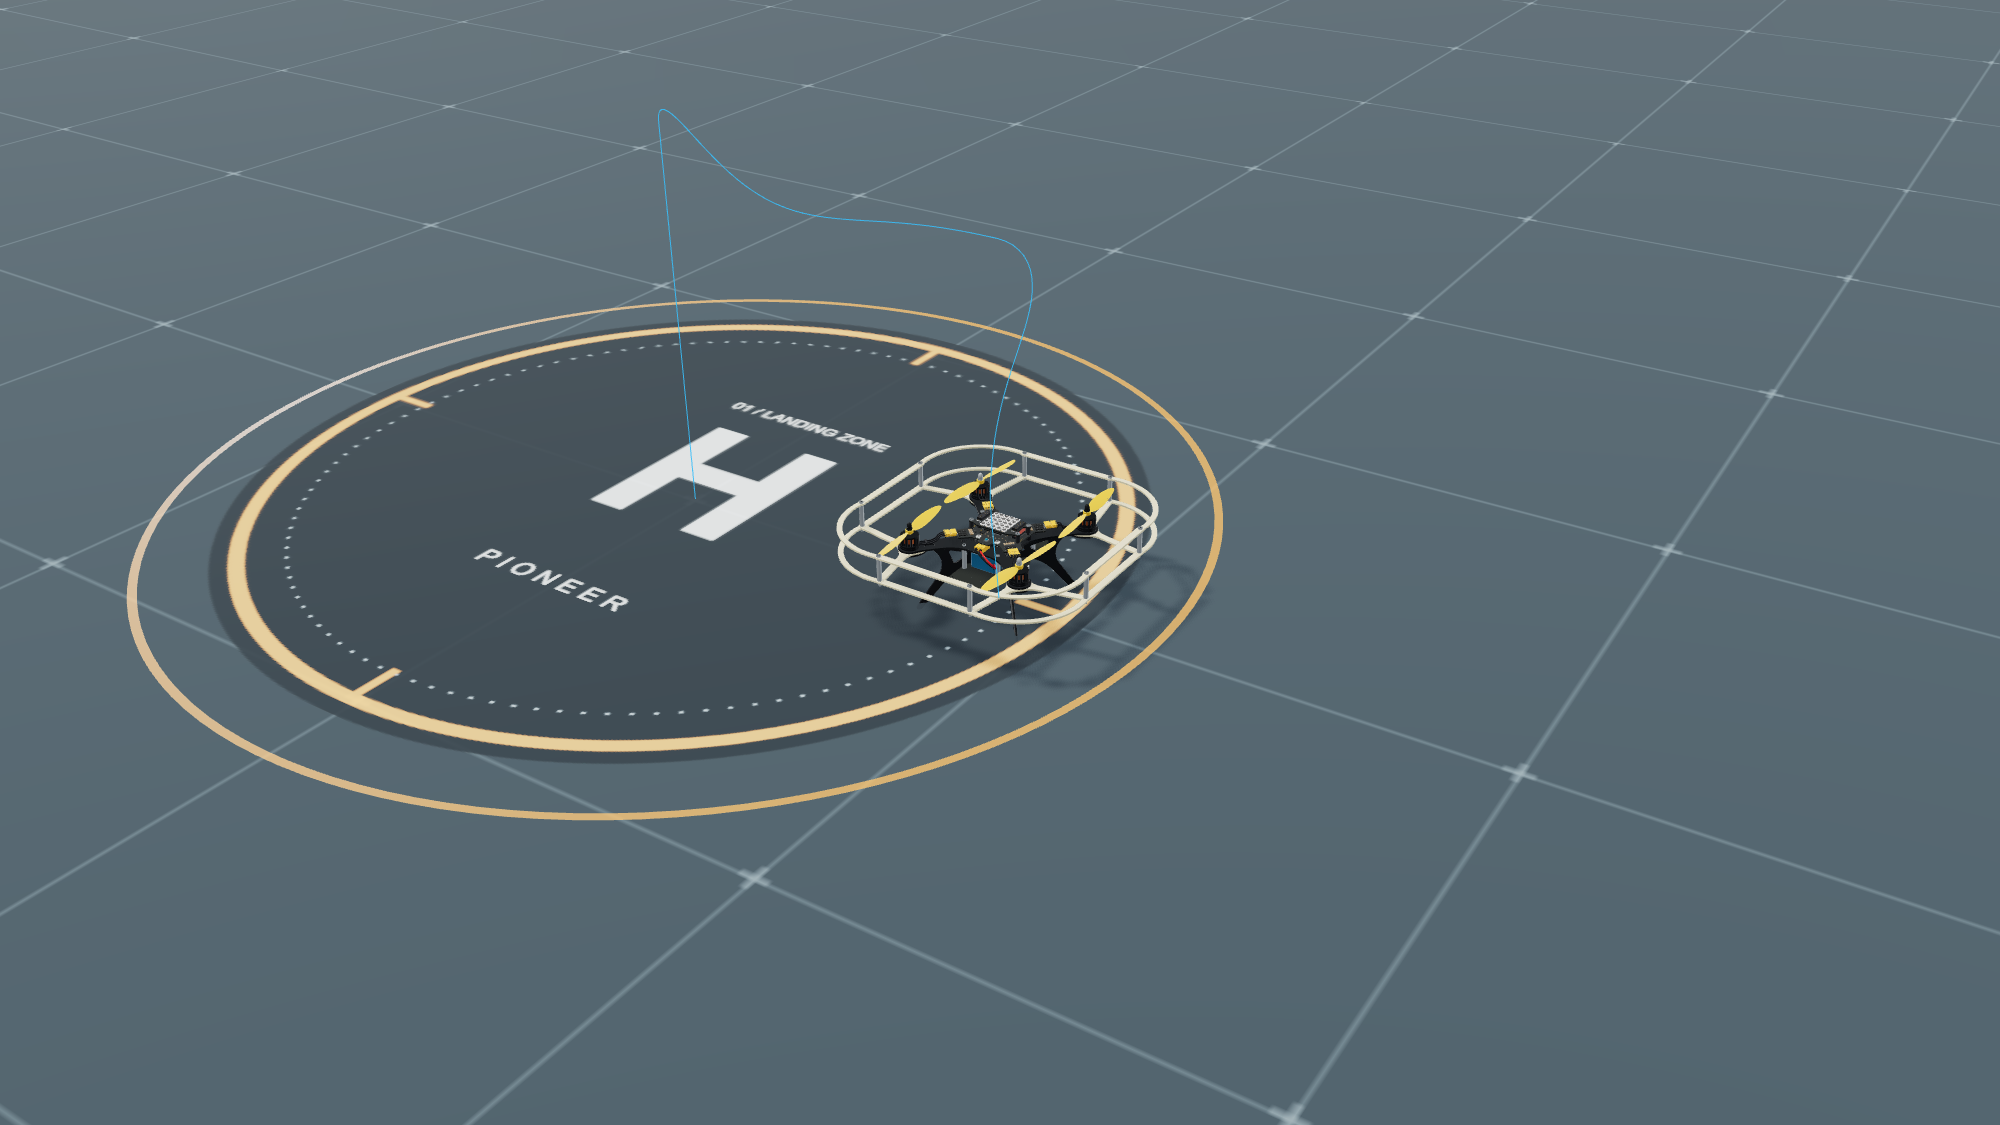
\includegraphics[width=136mm]{images/simulator/cover.png}};
        \end{tikzpicture}%
        \vspace{9.6cm}
        \titlechip{Lua}\hspace{4pt}\titlechip{Python}\hspace{4pt}\titlechip{Bricks}\hspace{4pt}\titlechip{SDK2 и RKNN}\hspace{4pt}\titlechip{ROS 2 и рой}\hspace{4pt}\titlechip{Симулятор}\par
        \vspace{0.5cm}
        {\small\color{Muted}\raggedright От первой строки кода до автономной миссии: язык, светодиоды и таймеры, события автопилота, полёт по точкам, камера и навигация по маркерам, нейросети на борту Пионера Мини~2, ROS~2 и групповой полёт. Каждый пример запускается в симуляторе и проверяется автоматически.\par}
        \vfill
        {\large\bfseries\color{Ink} #3\par}
        \vspace{3pt}
        {\small\color{Muted} #4\par}
        \vspace{0.45cm}
        {\color{Rule}\rule{\linewidth}{0.6pt}}\par
        \vspace{5pt}
        {\small\color{Ink} #5\hfill\texttt{simulator.sakoryagin.ru}\par}
        \vspace{2pt}
        {\footnotesize\color{Muted} Версия \theversion\ · сборка \buildtimestamp\par}
    \end{titlepage}
}
